\begin{definition}
	A Petrinet $\Omega$ is a directed graph $(V, E)$ with vertices $V=(V_x,
		V_z)$ partitioned into sets $V_x$ of state vertices and $V_z$ of transition
	vertices, and edges $E=(E_{out}, E_{in})$ partitioned into collections $E_{out}$ of
	flow-out and $E_{in}$ flow-in edges (relative to state vertices).
\end{definition}



\begin{definition}
	A flow-out edge $e \in E_{out}$ comprises a pair of vertices $(v_x,v_z)$, where
	$v_x \in V_x$ is a state vertex, $v_z \in V_z$ is a transition vertex, and the
	flow is directed from $v_x$ to $v_z$.
\end{definition}

\begin{definition}
	A flow-in edge $e \in E_{in}$ comprises a pair of vertices $(v_z,v_x)$,
	similar to a flow-out edge, except that the flow is directed from $v_z$ to
	$v_x$.
\end{definition}

\begin{example}
	The SIR model that stratifies the $S$ state variable into $S_1$ and $S_2$
	for two susceptible populations and defines $\Omega$ by:
	\begin{eqnarray*}
		V_x &=& \{v_{S_1}, v_{S_2}, v_{I}, v_{R}\}\\
		V_z &=& \{v_{inf_1}, v_{inf_2}, v_{rec}\}\\
		E_{in} &=& ((v_{inf_1}, v_{S_1}), (v_{inf_1}, v_{I}), (v_{inf_1}, v_{I}), (v_{inf_2}, v_{S_2}), (v_{inf_2}, v_{I}),
		(v_{inf_2}, v_{I}), (v_{rec}, v_{R}))\\
		E_{out} &=& ((v_{S_1}, v_{inf_1}), (v_{S_2}, v_{inf_2}),(v_{I}, v_{inf_1}), (v_{I}, v_{rec}))
	\end{eqnarray*}
\end{example}

\begin{figure}
	\centering    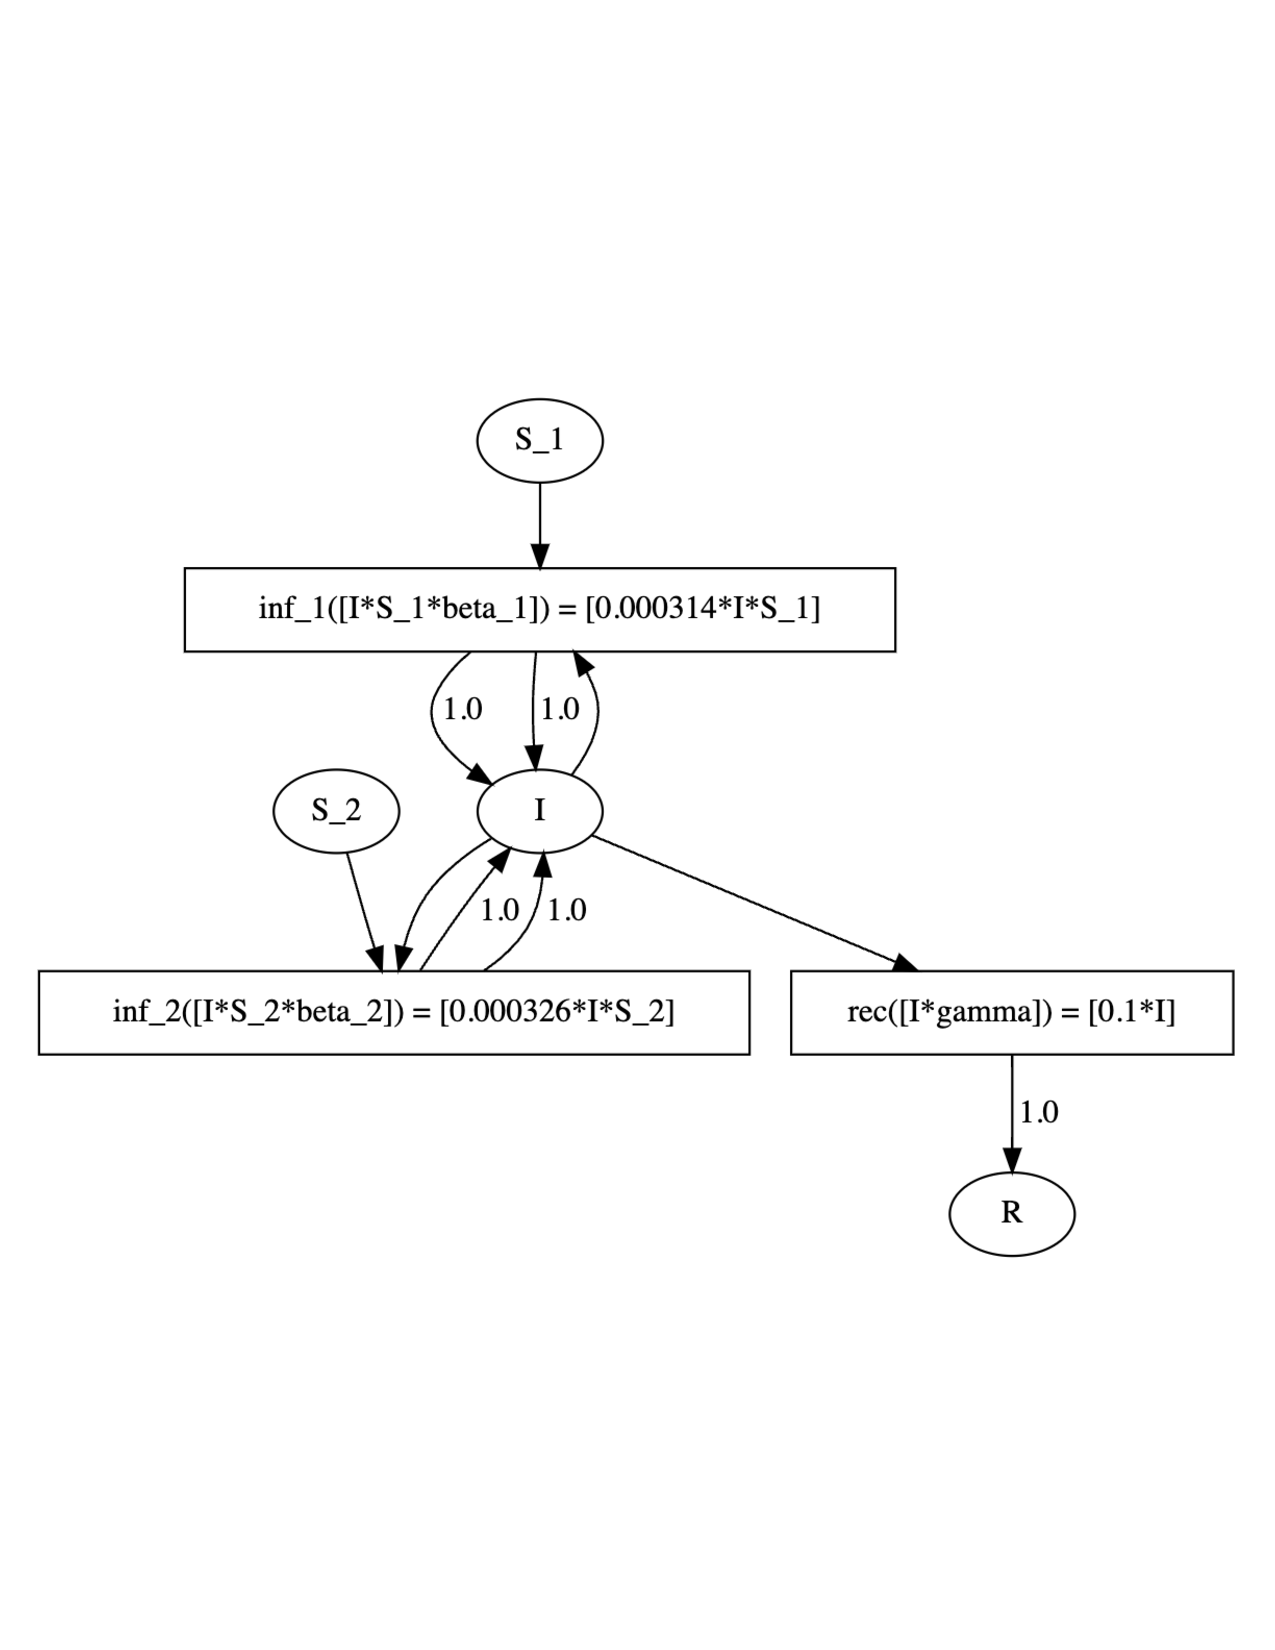
\includegraphics[width=.5\linewidth]{fig/sir/sir_stratified_model.pdf}
	\caption{\label{fig:sir_stratified_model} SIR model stratified with two
		populations in the $S$ state ($S_1$ and $S_2$), each with a unique $\beta$
		parameter ($\beta_1$ and $\beta_2$).}
\end{figure}

\begin{definition}
	The ODE semantics $\Theta$ of the Petrinet $\Omega$ defines a tuple $(P, X,
		Z, {\cal I}, {\cal P}, {\cal X}, {\cal Z}, {\cal R})$ where
	\begin{itemize}
		\item $P$ is a set of parameters;
		\item $X$ is a set of state variables;
		\item $Z$ is a set of transitions;
		\item ${\cal I}: S \rightarrow \reals$ assigns the initial value of
		      state variables to a real number;
		\item ${\cal P}: P \rightarrow \reals \cup \reals \times \reals$ assigns
		      parameters to a real number, or a pair of real numbers defining an
		      interval;
		\item ${\cal X}: X \rightarrow V_x$ assigns state variables to state
		      vertices;
		\item ${\cal Z}: Z \rightarrow V_z$ assigns transtions to transition
		      vertices; and
		\item ${\cal R}: {\bf P} \times {\bf X} \times Z \rightarrow \reals$
		      defines the rate of each transition  $z \in Z$ in terms of the set of
		      parameter vectors ${\bf P}$ and state variable vectors ${\bf X}$.
	\end{itemize}
	The elements of the Petrinet $\Omega$ and semantics $\Theta$ define the
	partial derivative $\frac{d {\bf x}}{dt}$, so that for each state variable
	$x \in X$:

	\begin{equation}\label{eqn:flow}
		\frac{dx}{dt} = \sum_{z \in Z^{in(x)}} {\cal R}({\bf p}, {\bf x}, z) - \sum_{z \in Z^{out(x)} } {\cal R}({\bf p}, {\bf x}, z)
	\end{equation}
	\noindent where $Z^{in(x)} = \{z \in Z | (z, x) \in E_{in}\}$ and
	$z^{out(x)}=\{z \in Z| (x, z) \in E_{out}\}$ are the transition
	vertices that flow in and out of the vertex $v_x$, respectively. We denote
	by $\nabla_{\Omega, \Theta}({\bf p}, {\bf x}, t) = (\frac{dx_1}{dt},
		\frac{dx_2}{dt}, \ldots)^T$, the gradient comprised of components defined in
	Equation \eqref{eqn:flow}.
\end{definition}

In the following, we simplify the definition of a Petrinet and associated
semantics because the graph vertices and the semantic elements are one to one.  We drop
the vertex terminology by assuming the following:
\begin{itemize}
	\item States: given $X$, $V_x$ and ${\cal X}$, referring to a state
	      variable $x \in X$ is synonymous with $v_x$ because ${\cal X}(x) = v_x$.
	\item Transitions: given $Z$, $V_z$ and ${\cal Z}$, referring to a state
	      variable $z \in Z$ is synonymous with $v_z$ because ${\cal Z}(z) = v_z$.
	\item Edges: Each edge $e \in E$ corresponds to a pair of vertices $(v_x,
		      v_z)$ or $(v_z, v_x)$, and it is (respectively) synonymous to pairs $(x, z)$
	      or $(z, x)$.
\end{itemize}

\begin{example}\label{ex:base}
	The stratified SIR model defines $\Theta$ (dropping ${\cal X}$ and ${\cal
				Z}$ per above) by:
	\begin{eqnarray*}
		P &=& \{\beta_1, \beta_2, \gamma\}\\
		X &=& \{S_1, S_2, I, R\}\\
		Z &=& \{inf_1, inf_2, rec\}\\
		{\cal I} &=& \left\{
		\begin{array}{ll}
			0.45 & :S_1 \\
			0.45 & :S_2 \\
			0.1  & :I   \\
			0.0  & :R
		\end{array}\right.\\
		{\cal P}&=& \left\{
		\begin{array}{ll}
			1e{-7} & :\beta_1 \\
			2e{-7} & :\beta_2 \\
			1e{-5} & :\gamma
		\end{array}\right.\\
		\\
		% {\cal X} &=& \left\{ 
		%     \begin{array}{ll}
		%         v_{x} & : x \in X
		%     \end{array}\right.\\
		% {\cal Z} &=& \left\{ 
		%     \begin{array}{ll}
		%         v_{z} & : z \in Z
		%     \end{array}\right.\\
		{\cal R} &=& \left\{
		\begin{array}{ll}
			\beta_1 S_1 I & : z_{inf_1} \\
			\beta_2 S_2 I & : z_{inf_2} \\
			\gamma I      & : z_{rec}   \\
		\end{array}\right.\\
	\end{eqnarray*}
\end{example}


Using the partial derivatives defined by the Petrinet graph and semantics, we
can define the state vector at given time $t+dt$ with the forward Euler method
as:

\begin{eqnarray*}
	\frac{d {\bf x}}{dt} &=& \nabla_{\Omega, \Theta}({\bf p},{\bf x}, t)\\
	\frac{{\bf x}(t+dt)-{\bf x}(t)}{dt} &=& \nabla_{\Omega, \Theta}({\bf p},{\bf x},
	t)\\
	{\bf x}(t+dt)&=& \nabla_{\Omega, \Theta}({\bf p},{\bf x}, t)dt+ {\bf x}(t)
\end{eqnarray*}


\begin{definition}
	The stratification $\text{Stratify}_{Q}(\Omega,
		\Theta) = (\Omega_Q, \Theta_Q)$ of a Petrinet and semantics  with
	respect to a specification $Q = (x, {\cal D}, P')$ defines a new Petrinet and
	semantics with the following properties:
	\begin{itemize}
		\item Parameters: For each $p \in P' \subseteq P$,
		\item States: For each element $D_i$ of the partition ${\cal D}= [D_0 | D_1| \ldots]$, define
		      $X' = X\backslash \{x\} \cup \{x_{D_i} |  {\cal D} = [D_0 | D_1| \ldots]\}$
		\item Transitions: For each transition $z \in Z^{in(x)}\cup Z^{out(x)}$
		      and partition $D_i$, define each $z_{D_i}$ so that:
		      \begin{itemize}
			      \item $E'_{in} = E_{in} \backslash \{(z, x)\} \cup \{(z_{D_i},
				            x_{D_i})| {\cal D} = [D_0 | D_1| \ldots]\}$ if $z \in
				            Z^{in(x)}$.
			      \item $E'_{out} = E_{out} \backslash \{(x, z)\} \cup \{(x_{D_i},
				            z_{D_i})| {\cal D} = [D_0 | D_1| \ldots]\}$ if $z \in
				            Z^{in(x)}$.
			      \item ${\cal R}({\bf p},{\bf x}, z_{D_i})$
		      \end{itemize}
		\item Initial State
		\item Parameter Values:
		\item Transition Rates:
	\end{itemize}
\end{definition}
